\NeedsTeXFormat{LaTeX2e}

\documentclass[10pt,a4paper]{article}
\usepackage{a4wide}
\usepackage{amssymb}
\usepackage{amsmath}
\usepackage{wrapfig}
\usepackage{graphicx}
\usepackage{color}
\usepackage{subfig}
\usepackage[english,ngerman]{babel}
\usepackage{listings}
\usepackage{url}
\usepackage[T1]{fontenc}
\usepackage[utf8]{inputenc}

\usepackage[authordate,bibencoding=auto,strict]{biblatex-chicago}
\usepackage[babel,german=guillemets]{csquotes}

\usepackage{hyperref}

\usepackage{todonotes}
\usepackage{xcolor}
\usepackage{array}

\newcolumntype{N}{@{}m{0pt}@{}}
\newcolumntype{M}[1]{>{\centering\arraybackslash}m{#1}}
\newcommand\litem[1]{\item{\bfseries #1\\}}
\newcommand\cRect[3]{{\color{#1}\rule{#2}{#3}}}

\definecolor{lightgray}{rgb}{.9,.9,.9}
\definecolor{darkgray}{rgb}{.4,.4,.4}
\definecolor{purple}{rgb}{0.65, 0.12, 0.82}
\definecolor{light-gray}{gray}{0.80}


\bibliography{Bibliography}



\setlength{\parindent}{0pt}
\setlength{\parskip}{5pt plus 2pt minus 1pt}

\lstdefinelanguage{JavaScript}{
  keywords={typeof, new, true, false, catch, function, return, null, catch, switch, var, if, in, while, do, else, case, break},
  keywordstyle=\color{blue}\bfseries,
  ndkeywords={class, export, boolean, throw, implements, import, this},
  ndkeywordstyle=\color{darkgray}\bfseries,
  identifierstyle=\color{black},
  sensitive=false,
  comment=[l]{//},
  morecomment=[s]{/*}{*/},
  commentstyle=\color{purple}\ttfamily,
  stringstyle=\color{red}\ttfamily,
  morestring=[b]',
  morestring=[b]"
}

\lstdefinelanguage{CSS}{
  morekeywords={color,background,margin, decorator},
  sensitive=false,
  morecomment=[l]{//},
  morecomment=[s]{/*}{*/},
  morestring=[b]",
}

\lstset{
   language=JavaScript,
   extendedchars=true,
   basicstyle=\footnotesize\ttfamily,
   showstringspaces=false,
   showspaces=false,
   numbers=left,
   numberstyle=\footnotesize,
   numbersep=9pt,
   tabsize=2,
   breaklines=true,
   showtabs=false,
   captionpos=b
}

\selectlanguage{ngerman}

\begin{document}
\listoftodos

\begin{titlepage}
\begin{center}


\includegraphics[width=5cm]{images/FHSLogo.pdf}

\vspace*{4cm}

\Large{
  \textit{\textbf{Bachelorarbeit 2}}
}

\vspace*{4cm}

\large{
  \textbf{Komponentenbasierte Softwarearchitektur und Softwareentwicklung: Ein Vergleich von Web-Components und Google Polymer}\\
}

\end{center}

\vfill

\begin{tabbing}
StudentIn \= \ Georg Eschbacher, 1110601005 \\
BetreuerIn \> \ Hubert Hölzl

\end{tabbing}

Salzburg, am 04. Mai 2014
\end{titlepage}


\pagestyle{headings}
\pagenumbering{roman}

\subsection*{Eidesstattliche Erklärung}
Ich erkläre hiermit eidesstattlich, dass ich die vorliegende Bachelorarbeit
selbständig und ohne fremde Hilfe verfasst, und keine anderen als die
angegeben Quellen und Hilfsmittel benutzt habe.
Weiters versichere ich hiermit, dass ich die den benutzten Quellen wörtlich
oder inhaltlich entnommenen Stellen als solche kenntlich gemacht habe.

Die Arbeit wurde bisher in gleicher oder ähnlicher Form keiner anderen
Prüfungskommission weder im In- noch im Ausland vorgelegt und auch nicht
veröffentlicht.

\vspace*{3cm}
Salzburg, am 05. Mai 2014\\
Datum
\hfill
Unterschrift


\newpage
\section*{Kurzfassung}
\begin{tabular}{l l}
Vor- und Zuname:& Vorname NACHNAME\\
Institution: & FH Salzburg\\ 
Studiengang: &  Bachelor MultiMediaTechnology\\ 
Titel der Bachelorarbeit: & Die Bachelorarbeit und ihre Folgen\\
Begutachter: & Titel Vorname Nachname\\ 
\end{tabular} 
\vspace{0.5cm}

Deutsche Zusammenfassung ...

... zwischen 150 und 300 Worte ...

\paragraph{Schlagwörter:}
Folgen, Bachelor, Wissenschaftliches Arbeiten


\newpage
\selectlanguage{english}
\subsection*{Abstract}
English abstract ...

... between 150 and 300 words ...

\todo[inline]{English Abstract}

\paragraph{Keywords:}
\textit{a few descriptive keywords}

\selectlanguage{ngerman}


\newpage
\tableofcontents

\newpage
\setcounter{page}{1}
\pagenumbering{arabic}

\section{Einleitung}
\label{sec:1_Einführung}

\subsection{Relevanz}
\label{sec:1_Relevanz}

Zu Beginn muss geklärt werden, wie eine Softwarekomponente im Allgemeinen definiert ist. 1996 wurde die Softwarekomponente bei der European Conference on Object-Oriented Programming (ECOOP) folgendermaßen definiert \citereset \autocite[siehe][S. 35-47]{Szyperski.2002}:
\begin{quote}
\glqq A software component is a unit of composition with contractually specified interfaces and explicit context dependencies only. A software component can be deployed independently and is subject to composition by third parties.\grqq
\end{quote}
Um dies näher erläutern zu können, wird ein gängiger Tätigkeitsbereich eines Softwarearchitekten herangezogen: das Erstellen einer Liste von Komponenten, die in die gesamte Software-Architektur problemlos eingefügt werden kann. Diese Liste gibt dem Entwicklungsteam vor, welche Komponenten das Softwaresystem zum Schluss umfassen wird. In einfachen Worten zusammengefasst sind Softwarekomponenten die Teile, die eine Software definieren \citereset \autocite[siehe][S. 35-47]{Szyperski.2002}.

Komponentenentwicklung bezeichnet die Herstellung von Komponenten, die eine spezielle Funktion in einer Softwarearchitektur übernehmen. Sämtliche Komponenten sollten immer für sich gekapselt und unabhängig voneinander sein. Dies garantiert die Wiederverwendbarkeit von bereits entwickelten Komponenten. Mehrere Komponenten werden mit Hilfe eines Verbindungsverfahrens zusammengeführt, beziehungsweise verwendet.

Softwarekomponenten haben ihren Ursprung im \glqq Unterprogramm\grqq . Ein \glqq Unterprogramm\grqq , oder auch \glqq Subroutine\grqq\ genannt, ist der Teil einer Software, der von anderen Programmen beziehungsweise Programmteilen aufgerufen werden kann. Eine Subroutine gilt als Ursprung der ersten Einheit für die Softwarewiederverwendung \citereset \autocite[siehe][]{Wheeler.1985}.

Programmiererinnen und Programmierer entdeckten, dass sie sich auf die Funktionalität von zuvor geschriebenen Codesegmenten berufen können, ohne sich beispielsweise um ihre Implementierung kümmern zu müssen. Neben der Zeitersparnis, die dadurch entstand, erweiterte diese \glqq Technik\grqq\ die Denkweisen: Der Fokus beim Entwickeln kann auf neue Algorithmen und komplexere Themen gelegt werden \citereset \autocite[siehe][S. 3-12]{Szyperski.2002}.

In der gleichen Weise, wie die frühen Subroutinen die Programmiererinnen und Programmierer vom Nachdenken über spezifische Details befreit haben, verschiebt sich durch komponentenbasierte Softwareentwicklung der Schwerpunkt von direkter Programmiersoftware zu komponierten Softwaresystemen, also komponentenbasierten Systemen. Das heißt, dass sich der Schwerpunkt in Richtung Integration von Komponenten verlagert hat. Darauf basiert die Annahme, dass es genügend Gemeinsamkeiten in großen Softwaresystemen gibt, um die Entwicklung von wiederverwendbaren Komponenten zu rechtfertigen. Diese Komponenten können dann auf Grund ihrer Gemeinsamkeiten für weitere Systeme genützt werden. Derzeit werden Komponenten gesucht, die eine große Sammlung von Funktionen bereitstellen. Für Unternehmen werden beispielsweise nicht nur simple Adressbücher, sondern ganze CRM-Systeme\footnote{Ein \glqq Customer Relationship Management System\grqq\ bezeichnet ein System, das zur Kundenpflege beziehungsweise Kundenkommunikation dient.} gesucht, um die Daten beziehungsweise Kommunikationen seiner Kunden zu sichern. Darüber hinaus sollten diese Systeme auch flexibel sein, d.h. es sollte mit anderen Komponenten erweitert werden können \citereset \autocite[siehe][S. 17-25]{Andresen.2003}.

Komponentenbasierte Entwicklung dient des Weiteren der Verwaltung von Komplexität innerhalb eines Systems. Sie versucht die Komplexität gering zu halten, indem die Programmiererin und der Programmierer sich vollständig auf die Implementierung der Komponenten fokussieren können. Das Verknüpfen beziehungsweise Kombinieren von Komponenten sollte demnach nicht mehr Aufgabe der Entwicklerin und des Entwicklers sein. Um diese Aufgabe zu lösen wird ein Architektur-Framework\footnote{Ein Komponenten-Architektur-Framework basiert auf einer Reihe von Plattform Entscheidungen, einer Reihe von Komponenten-Frameworks und ein Interoperabilitätsdesign der Komponenten-Frameworks \citereset \autocite[siehe][419-422]{Szyperski.2002}.} eingesetzt, das Aktivitäten zur Identifikation, Spezifikation, Realisierung und Verteilung von Komponenten beschreibt. Vorteile durch dieses Programmierparadigma sind somit einerseits die Zeitersparnisse und andererseits die erhöhte Qualität der Komponenten \citereset \autocite[siehe][S. 1-3]{Andresen.2003}. Standardmäßig werden in einem Softwaresystem Annahmen über den Kontext impliziert, in dem das System funktioniert. Die komponentenbasierte Softwareentwicklung verlangt,
\begin{quote}
  \glqq[\dots], dass all diese Annahmen explizit definiert werden, damit das System in verschiedenen Kontexten wiederverwendet werden kann \citereset \autocite[siehe][]{Andresen.2003}.\grqq
\end{quote}

Durch diese explizite Definition von Annahmen gibt es verschiedene Anwendungsszenarien, die automatisch als Testszenarien der Komponenten dienen.

Im Zeitalter von Internet, Intranet und Extranet sind viele verschiedene Systeme und Komponenten miteinander zu verbinden. Aus den folgenden Gründen ist eine erweiterbare und flexible Architektur notwendig, die eine schnelle Reaktion auf neue Anforderungen ermöglicht: Web-basierte Lösungen sollen auf Informationen eines Servers zugreifen können, um z.B. mittels eines Extranets diversen Händlern transparente Einblicke in die Lagerbestände eines Unternehmens zu ermöglichen. ERP\footnote{Enterprise Resource Planning}- und CRM-Systeme sollen eingebunden werden, um die Betreuung und den Service für Kunden optimieren zu können \citereset \autocite[siehe][S. 39-42]{Andresen.2003}.

Um diesen Anforderungen gerecht zu werden, gab es in den letzten Jahren eine unüberschaubare Anzahl an Frameworks beziehungsweise Bibliotheken, die die Entwicklung von Komponenten vereinfachten. Das Problem hierbei war, dass die Komponenten, die mit Hilfe der Frameworks beziehungsweise Bibliotheken entstanden sind, nicht mit anderen Frameworks beziehungsweise Bibliotheken verknüpft werden konnten. Eine Standardisierung, wie Komponenten im Web-Bereich aussehen müssen beziehungsweise wie die Schnittstellen definiert sein müssen, um Wiederverwendbarkeit garantieren zu können, gab es bis dato nicht. Eine neue Technologie, die zurzeit vom W3C standardisiert wird, gehört zu den interessantesten Webtechniken, da sie eine Standardisierung für Komponenten im Web-Bereich bieten. Diese Technologie versucht eine Vielzahl von Funktionen der populärsten JavaScript-Komponentenframeworks aufzunehmen und nativ in den Browser zu portieren. Dadurch wird es möglich, benutzerdefinierte Komponenten und Applikationen entwickeln zu können, ohne dabei zahlreiche andere Bibliotheken einbinden zu müssen. Weiters wird durch die Standardisierung die Wiederverwendbarkeit beziehungsweise Interoperabilität von Komponenten gewährleistet.



\subsection{Motivation}
\label{sec:1_Motivation}

Die persönliche Motivation zu diesem Thema entstand grundsätzlich in der Zeit eines Praktikums des Autors. Hier war es erforderlich, Front-End Komponenten für verschiedene Web-Applikationen zu entwickeln. Grundanforderung der Komponenten war, dass sie wiederverwendet werden können. Hauptproblem bei der Entwicklung der Komponenten war, dass die Web-Applikationen auf unterschiedlichen Frameworks basierten und sämtliche Komponenten immer an den \glqq Standard\grqq\ der Frameworks angepasst werden mussten.

Web-Components bietet als erste Technologie einen allgemeinen Standard für Komponenten im Web-Bereich, wodurch sie für mich sehr interessant ist. Dadurch, dass Web-Components jedoch noch unter schlechter Browser-Unterstützung leiden, wird in dieser Arbeit auch der Polyfill Polymer von Google näher analysiert. Polymer versucht jegliche Funktionen von Web-Components im Browser zu emulieren, um sie somit für sämtliche \glqq Evergreen\grqq -Browser zur Verfügung stellen zu können.

Ein weiterer Punkt der persönlichen Motivation des Autors ist die grundsätzliche Änderung beziehungsweise Erweiterung einiger Konzepte der Web-Entwicklung durch Web-Components. Durch die vollständige Kapselung von Komponenten können keine Abhängigkeitsprobleme untereinander mehr entstehen. Beispielsweise hierfür sind unterschiedliche jQuery-Versionen unter den Komponenten. Auch ist das erstellen von Custom-Elements eine große Änderung. Das Markup von Komponenten kann zukünftig mit Hilfe eines benutzerdefinierten Tags gerendert werden. Dies hilft vor allem bei Komponenten, die sehr darstellungsabhängig sind.

Auf Grund des bereits zuvor genannten Hauptproblems bei der Entwicklung von Komponenten wird auch ein Praxisprojekt im Zuge der Bachelorarbeit erstellt. Hierbei wird der Fokus auf die Programmierung von zwei wiederverwertbaren Frontend-Oberflächen gelegt. Zum einen wird eine Diagramm-Komponente und zum anderen ein komplexes Menü entwickelt, dass für spätere Projekte weiterverwendet werden kann. Die Hauptanforderung ist einerseits die Kompatibilität zu so vielen Browsern wie möglich zu gewährleisten und andererseits die Interoperabilität mit anderen Komponenten sicherzustellen. Des Weiteren soll durch die einmalige Programmierung dieser Komponente und deren darauffolgende Wiederverwendung der Wartungsaufwand möglichst gering gehalten werden. Somit wird in dieser Arbeit geklärt, inwiefern die Entwicklung von Web-Components ohne Unterstützungen wie beispielsweise das Polymer Projekt bereits möglich ist. Weiterhin soll geklärt werden, welche Aspekte der klassischen Softwarearchitektur bei der Entwicklung von Web-Components aufgegriffen werden und inwiefern es mit komponentenbasierter Softwareentwicklung beziehungsweise komponentenbasierter Softwarearchitektur vereinbar ist. Folgend werden diese Aspekte nicht nur an Hand der zur Zeit standardisierten Technologie namens Web-Components analysiert, sondern auch an Hand des von Google zur Verfügung gestellten Polyfills namens Polymer.


\subsection{Forschungsfrage}
\label{sec:1_Forschungsfrage}
In dieser Arbeit soll folgende Forschungsfrage geklärt werden:
\begin{quote}
Welche Aspekte greifen Web Components aus der komponentenbasierten Softwarearchitektur auf und welche Vor- und Nachteile bietet dabei das Google Polymer Projekt.
\end{quote}


\subsection{Struktur der Arbeit}
\label{sec:1_Struktur}

\todo[inline]{Anpassen (mit neuen Kapitel etc.)}

Die Arbeit beginnt mit einer allgemeinen Einführung zu den Begriffen \glqq Softwarearchitektur\grqq\ und \glqq Softwarekomponenten\grqq\ (siehe Kapitel \ref{sec:2_Softwarekomponente_Klassisch} auf Seite \pageref{sec:2_Softwarekomponente_Klassisch}). Nach dieser Erklärung werden die verschiedenen Arten von Softwarekomponenten aufgezeigt und näher erläutert (siehe Kapitel \ref{sec:2_Arten_Komponenten} auf Seite \pageref{sec:2_Arten_Komponenten}). Folgend wird der bereits erklärte Begriff der Softwarearchitektur (siehe Kapitel \ref{sec:2_Softwarearchitektur} auf Seite \pageref{sec:2_Softwarearchitektur}) auf zwei Teilbereiche beschränkt: einerseits die serviceorientierte Softwarearchitektur (siehe Kapitel \ref{sec:2_Serviceorientierte_Softwarearchitektur} auf Seite \pageref{sec:2_Serviceorientierte_Softwarearchitektur}) und andererseits die komponentenbasierte Softwarearchitektur (siehe Kapitel \ref{sec:2_Komponentenbasierte_Softwarearchitektur} auf Seite \pageref{sec:2_Komponentenbasierte_Softwarearchitektur}). Als Abschluss des Kapitels wird der feine Unterschied zwischen einem Dienst und einer Komponente näher erläutert (siehe Kapitel \ref{sec:2_Unterschied_Dienst_Komponente} auf Seite \pageref{sec:2_Unterschied_Dienst_Komponente}).

Das darauffolgende Kapitel bietet zu Beginn einen Überblick über Web-Components (siehe Kapitel \ref{sec:3_W3C} auf Seite \pageref{sec:3_W3C}). Weiters wird die Spezifikation dieser Technologien an Hand einiger Beispiele näher erläutert (beginnend bei Kapitel \ref{sec:3_WC_Templates} auf Seite \pageref{sec:3_WC_Templates} ff.). Auf Grund der mangelnden Browser-Unterstützung von Web-Components (siehe Kapitel \ref{sec:3_WC_Support} auf Seite \pageref{sec:3_WC_Support}) wird folglich Google-Polymer vorgestellt. Dieses Projekt soll sämtliche \glqq Evergreen\grqq -Browser unterstützen (siehe Kapitel \ref{sec:4_Polymer_Support} auf Seite \pageref{sec:4_Polymer_Support}) und somit die Entwicklung mit Web-Components Technologien bereits ermöglichen. Das Framework wird in Kapitel \ref{sec:4_Polymer} auf Seite \pageref{sec:4_Polymer} genauer erklärt.

In Kapitel \ref{sec:5_Vergleich_WC_Polymer} auf Seite \pageref{sec:5_Vergleich_WC_Polymer} wird ein detaillierter Vergleich von Web-Components und Polymer erstellt. Dieser Vergleich beinhaltet Aspekte beziehungsweise Relationen zur klassischen Softwareentwicklung (siehe Kapitel \ref{sec:5_Vergleich_Architektur} auf Seite \pageref{sec:5_Vergleich_Architektur}), serviceorientierten Softwarearchitektur (siehe Kapitel \ref{sec:5_Vergleich_SOA} auf Seite \pageref{sec:5_Vergleich_SOA}), komponentenbasierten Softwarearchitektur (siehe Kapitel \ref{sec:5_Vergleich_CBA} auf Seite \pageref{sec:5_Vergleich_CBA}) und komponentenbasierten Softwareentwicklung (siehe Kapitel \ref{sec:5_Vergleich_CBSE} auf Seite \pageref{sec:5_Vergleich_CBSE}).

Als Praxisprojekt der Arbeit wurden zwei Komponenten definiert: eine Diagramm-Komponente und eine Menükomponente. Beide Komponenten werden zum einen mit Hilfe von nativen Technologien und zum anderen mit Hilfe von Google-Polymer umgesetzt (siehe Kapitel \ref{sec:6_WC_Pur} auf Seite \pageref{sec:6_WC_Pur} und Kapitel \ref{sec:6_WC_Polymer} auf Seite \pageref{sec:6_WC_Polymer}).

Die bis zu diesem Zeitpunkt definierten Begriffe und Erkenntnisse werden im Abschlusskapitel der Arbeit nochmal aufgegriffen und kurz beschrieben (siehe Kapitel \ref{sec:5_Konklusion} auf Seite \pageref{sec:5_Konklusion}). Abschließend wird der Ausblick sowie noch offene Fragen dieser Arbeit geklärt.
\section{Softwarearchitektur und Softwarekomponenten}
\label{sec:2_Architektur}
Das Kapitel \ref{sec:2_Architektur} sollte der Leserin und dem Leser verhelfen, den Begriff \glqq Softwarearchitektur\grqq\ zu verstehen. Demnach sollen Vorteile von der Verwendung von Softwarearchitektur genannt werden. Des Weiteren werden wichtige Begriffe wie serviceorientierte Architektur beziehungsweise komponentenbasierte Softwarearchitektur näher erläutert.
Auch wird in Kapitel \ref{sec:2_Architektur} nur Architektur behandelt, die sich über die Erstellung, Auslieferung und den Betrieb von Software jeglicher Art erstreckt. Folglich gibt es Berührungspunkte zu anderen Architektur-Arten wie zum Beispiel der Daten- oder Sicherheitsarchitektur, die jedoch nicht in dieser Arbeit behandelt werden.

\subsection{Klassische Softwarekomponente}
\label{sec:2_Softwarekomponente_Klassisch}
\begin{quote}
\glqq The characteristic properties of a component are that it:
\begin{itemize}
\item is a unit of independent deployment
\item is a unit of third-party composition
\item has no (externally) observable state\grqq
\end{itemize}
\end{quote}

Dies ist die Definition einer Komponente von Clemens Szyperski im Buch \glqq Component software: Beyond object-oriented programming\grqq \citereset \autocite{Szyperski.2002}.
Diese Definition bedarf weiterer Erläuterung.
\begin{description}
\item[A component is a unit of independent deployment] \hfill \\
Dieser Punkt der Definition besitzt eine softwaretechnische Implikation. Damit eine Komponente \glqq independent deployable\grqq\ also unabhängig auslieferbar ist, muss sie auch so konzipiert beziehungsweise entwickelt werden. Sämtliche Funktionen der Komponente müssen vollständig unabhängig von der Verwendungsumgebung und von anderen Komponenten sein. Des Weiteren muss der Begriff \glqq independent deployable\grqq\ als Ganzes betrachtet werden, denn es bedeutet, dass eine Komponente nicht partiell, sondern nur als Ganzes ausgeliefert wird. Ein Beispiel für diesen Kontext wäre, dass ein Dritter keinen Zugriff auf die involvierten Komponenten einer Software hat.\\
\item[A component is a unit of third-party composition] \hfill \\
Hier wird der Begriff \glqq composable\grqq\ dahingehend verstanden, dass Komponenten zusammensetzbar sein sollen. In diesem Kontext bedeutet dies, dass eine Applikation aus mehreren Komponenten bestehen kann. Des Weiteren soll auch mit einer Komponente interagiert werden können, was einer klar definierten Schnittstelle bedarf. Nur mit Hilfe dieser Schnittstelle kann garantiert werden, dass die Komponente einerseits vollständig gekapselt von anderen Komponenten ist und andererseits mit der Umgebung interagieren kann. Dies erfordert demnach eine klare Spezifikation, was die Komponente erfordert und was sie bietet.
\item[A component has no (externally observable) state] \hfill \\
Eine Komponente sollte keinen (externen) \glqq observable\grqq also feststellbaren Zustand haben. Die Originalkomponente darf nicht von Kopien ihrer selbst unterschiedlich sein. Wenn Komponenten einen feststellbaren Zustand haben dürften, wäre es nicht möglich, zwei \glqq gleiche\grqq\ Komponenten mit den gleichen Eigenschaften zu haben. Eine mögliche Ausnahme von dieser Regel sind Attribute, die nicht zur Funktionalität der Komponente beitragen. Ein Beispiel in diesem Kontext wäre die Seriennummer für die Buchhaltung. Dieser spezifische Ausschluss ermöglicht einen zulässigen technischen Einsatz eines Zustands, der kritisch für die Leistung sein könnte. Beispielsweise dafür sei der Cache. Eine Komponente kann einen Zustand mit der Absicht zu cachen verwenden. \todo{umschreiben!}Ein Cache ist ein Speicher, auf den man ohne Konsequenzen verzichten kann, jedoch möglicherweise reduzierte Leistung in Anspruch nimmt.
\end{description}

In vielen aktuellen Ansätzen sind Komponenten eine schwerwiegende Einheit mit genau einer Instanz in einem System. Beispielsweise könnte ein Datenbankserver eine Komponente darstellen. Oftmals wird der Datenbankserver im Zusammenhang mit der Datenbank als Modul mit einem feststellbaren Zustand angesehen. Dahingehend ist der Datenbankserver ein Beispiel für eine Komponente und die Datenbank ein Beispiel für das Objekt, das von der Komponente verwaltet wird. Es ist wichtig zwischen dem Komponentenkonzept und dem Objektkonzept zu differenzieren, da das Komponentenkonzept in keinster weise den Gebrauch von Zuständen von Objekten fördert beziehungsweise zurückstuft \citereset \autocite{Szyperski.2002}.

Eine Softwarearchitektur ist die zentrale Grundlage einer skalierbaren Softwaretechnologie und ist für komponentenbasierte Systeme von größter Bedeutung. Nur da, wo eine Gesamtarchitektur mit Wartbarkeit definiert ist, finden Komponenten die Grundlage, die sie benötigen. Folgend werden einige Eckpfeiler einer Komponentenarchitektur genannt \citereset \autocite{Szyperski.2002}:
\begin{itemize}
\item Interaktionen zwischen Komponenten und deren Umfeld sind geregelt
\item Die Rollen von Komponenten sind definiert
\item Schnittstellen von Komponenten sind standardisiert
\item Aspekte der Benutzeroberflächen für Endbenutzer und Assembler sind geregelt
\end{itemize}
In Kapitel \ref{sec:2_Softwarearchitektur} auf Seite \pageref{sec:2_Softwarearchitektur} wird der Begriff der Softwarearchitektur näher erläutert. Des Weiteren werden in Kapitel \ref{sec:2_Serviceorientierte_Softwarearchitektur} auf Seite \pageref{sec:2_Serviceorientierte_Softwarearchitektur} und Kapitel \ref{sec:2_Komponentenbasierte_Softwarearchitektur} auf Seite \pageref{sec:2_Komponentenbasierte_Softwarearchitektur} zwei Aspekte der Softwarearchitektur hinsichtlich der Entwicklung mit Komponenten erklärt.



\subsection{Arten von Softwarekomponenten}
\label{sec:2_Arten_Komponenten}

Verschiedene Arten von Komponenten können entsprechend ihren Aufgabenbereichen klassifiziert werden. Eine übersichtliche Art der Zuordnung von Aufgabenbereichen zu Komponenten kann auf der Basis der Trennung von Zuständigkeiten erfolgen, zum Beispiel auf der Basis einer Schichten-Architektur. Eine Schichtenarchitektur dient der Trennung von Zuständigkeiten und einer losen Kopplung der Komponenten. Sie unterteilt ein Software-System in mehrere horizontale Schichten, wobei das Abstraktionsniveau der einzelnen Schichten von unten nach oben zunimmt. Eine jede Schicht bietet der über ihr liegenden Schicht Schnittstellen an, über die diese auf sie zugreifen kann. Abbildung \ref{fig:2_Schichtenarchitektur} auf Seite \pageref{fig:2_Schichtenarchitektur} veranschaulicht die bereits genannte Architektur \citereset \autocite{Andresen.2003}.
\begin{figure}[h]
\centering
%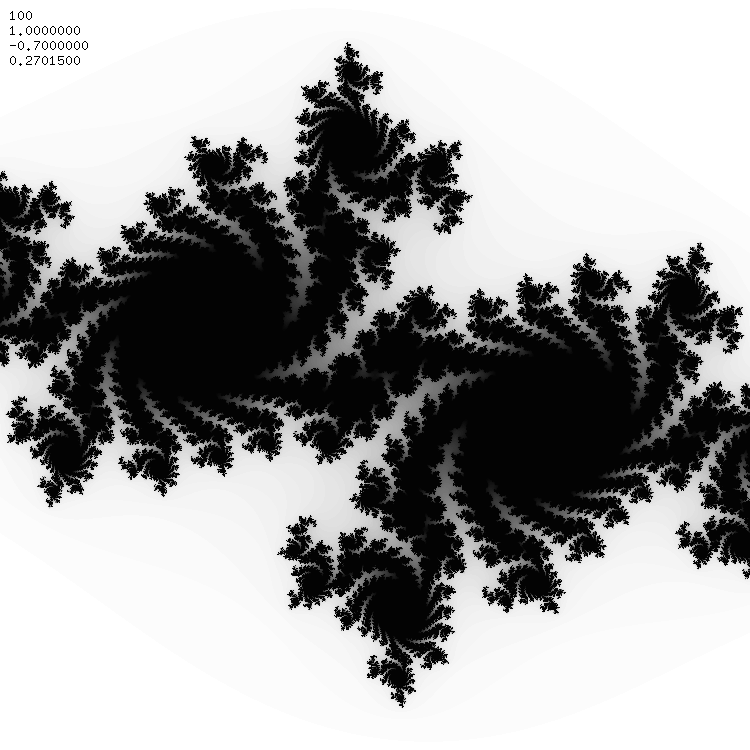
\includegraphics[height=5.0cm]{images/Julia-Fractal.png}
\missingfigure{Schichtenarchitektur}
\caption[
Beispiel einer Schichtenarchitektur, Urldate: 04.2014 \newline
%\small\texttt{http://upload.wikimedia.org/wikipedia/commons/e/e1/SchichtenarchitekturAufrufstrukturen.svg}
]{Beispiel einer Schichtenarchitektur}
\label{fig:2_Schichtenarchitektur}
\end{figure}





Auf Grundlage der in Abbildung \ref{fig:2_Schichtenarchitektur} auf Seite \pageref{fig:2_Schichtenarchitektur} veranschaulichten Architektur können Komponenten wie folgt unterteilt werden:
\begin{description}
\item[Komponenten der Präsentations-Schicht] \hfill \\
Diese Komponenten stellen eine nach außen sichtbare Benutzerschnittstelle dar. Ein Beispiel dieser Schnittstelle ist eine GUI\footnote{Graphical User Interface}-Komponente (Button, Menü, Slider, und vieles mehr\ldots).
\item[Komponenten der Controlling-Schicht] \hfill \\
Diese verarbeiten komplexe Ablauflogik und dienen als Vermittler zwischen Komponenten der Business- und Präsentations-Schicht.Beispielhaft hierfür wäre ein Workflow-Controller. Er koordiniert die Interaktion mit einer oder mehreren Businesskomponenten. Diese Komponente kann zum Beispiel den Ablauf eines Geschäftsprozesses umsetzen.
\item[Komponenten der Business-Schicht] \hfill \\
Sie bilden die Geschäftslogik im Sinne autonomer Businesskonzepte ab. Geschäftslogik in diesem Kontext bedeutet, dass die Komponente die Logik besitzt, die die eigentliche Problemstellung löst. Oftmals bezeichnet man hier die sogenannte Entity-Komponente. Sie dient der Perstistierung von Daten beziehungsweise bildet Entitäten auf Komponenten ab (Firma, Produkt, Kunden).
\item[Komponenten der Integrations-Schicht] \hfill \\
Sie dient der Anbindung an Alt-Systeme, Fremd-Systeme und Datenspeicher. Dies könnten eispielsweise Connector-Komponenten oder Datenzugriffs-Komponenten sein. Connector-Komponenten dienen der Integration eines Fremd-Systems und Datenzugriffs-Komponenten liefert den Datenzugriff für Komponenten der oben genannten Schichten. Bei Datenzugriffs-Komponenten werden die Besonderheiten einer Datenbank berücksichtigt.
\end{description}

\subsection{Softwarearchitektur}
\label{sec:2_Softwarearchitektur}

Architektur ist nicht ausschließlich eine technologische Angelegenheit, sondern beinhaltet zahlreiche soziale und organisatorische Gesichtspunkte, die den Erfolg einer Architektur und damit eines gesamten Projekts erheblich beeinflussen können. Wenn man bedenkt, dass Architektur in verschiedenen Bereichen ein Thema ist und unterschiedliche Aspekte bei der Erstellung eines Systems umfasst, wird deutlich, warum eine allgemeingültige Definition schwer fällt \citereset \autocite{Vogel.2009}.\\
Zu Beginn wird die klassische Architektur als Ausgangspunkt verwendet. Eine mögliche Definition der klassischen Architektur bietet das \glqq American Heritage Dictionary\footnote{Siehe \href{http://ahdictionary.com/word/search.html?q=architecture&submit.x=39&submit.y=20}{American Heritage Online-Dictionary}}\grqq :
\begin{quote}
  Architecture is:
  \begin{enumerate}
    \item The art and science of designing and erecting buildings.
    \item A style and method of design and construction
    \item Orderly arrangement of parts
  \end{enumerate}
\end{quote}

Wenn man diese Definition zugrunde legt, ist Architektur sowohl eine Kunst als auch eine Wissenschaft, die sich sowohl mit dem Entwerfen als auch mit dem Bauen von Bauwerken beschäftigt. Sie konzentriert sich nicht nur auf die Planung, sondern erstreckt sich bis hin zu der Realisierung eines Bauwerks. Ferner ist ein Schlüsselergebnis der Architekturtätigkeit das Arrangieren von Teilen des Bauwerks. Laut dieser Definition ist Architektur hiermit nicht nur die Struktur eines Bauwerks, sondern auch die Art und Weise, an etwas heranzugehen. Generell entstehen Architekturen auf Grund von Anforderungen, wie beispielsweise der Wunsch nach einer Behausung und unter Verwendung von vorhandenen Mitteln wie zum Beispiel Werkzeugen. Historisch basiert der eigentliche Entwurf auf dem Prinzip von Versuch und Irrtum. Erst durch die gewonnenen Architektur-Erfahrungen, welche mündlich oder schriftlich weitergegeben wurden, entwickelten sich Architekturstile. Folglich basiert Architektur auf Konzepten beziehungsweise Methoden, die sich in der Vergangenheit bewährt haben \citereset \autocite{Vogel.2009}.\\

Zum Begriff \glqq Architektur\grqq\ in der IT existieren im Gegensatz zur klassischen Architektur unzählige Definitionen\footnote{Das Software Engineering Institute(SEI) der Carnegie-Mellon Universität der Vereinigten Staaten von Amerika hat in der Fachliiteratur über 50 verschieene Definitionen für den Begriff \glqq Softwararchitektur\grqq\ ausgemacht.\href{http://www.sei.cmu.edu/architecture/definitions.html}{Software Architecture Definitions}}. Daran zeigt sich, dass es eine Herausforderung darstellt, eine Definition zu finden, die allgemein anerkannt wird \citereset \autocite{Shaw.1996}.

Softwarearchitektur erstreckt sich von der Analyse des Problembereichs eines Systems bis hin zu seiner Realisierung. Sie bewegt sich nicht auf der Abstraktionsebene fein-granularer Strukturen wie Klassen oder Algorithmen, sondern vielmehr auf der Ebene von Systemen, also grob-granularer Strukturen. Oftmals werden bei Projekten keine Aufwände im Zusammenhang mit Architektur bezahlt, was dazu führt, dass es im späteren Verlauf der Entwicklung zu vermeidbaren höheren finanziellen Kosten auf Grund eines erhöhten Wartungsaufwands kommen kann \citereset \autocite{Vogel.2009}.

\begin{description}
\item[Symptome mangelhafter Softwarearchitektur] \hfill \\
Fatalerweise zeigen sich die Folgen einer mangelhaften Architektur in der IT nicht selten erst mit erheblicher Verzögerung, das heißt, ernste Probleme treten eventuell erst auf, wenn ein System zum ersten Mal produktiv eingesetzt wird oder wenn es bereits im Einsatz ist und für neue Anforderungen angepasst werden muss. Eine Architektur, die ungeplant entstanden ist, sich also unbewusst im Laufe der Zeit entwickelt hat, führt zu erheblichen Problemen während der Erstellung, der Auslieferung und dem Betrieb eines Systems. Folgende Symptome können potentiell auf eine mangelhafte Architektur hindeuten \citereset \autocite{Vogel.2009}:
\begin{itemize}
\item Fehlender Gesamtüberblick
\item Komplexität ufert aus und ist nicht mehr beherrschbar
\item Planbarkeit ist erschwert
\item Risikofaktoren frühzeitig erkennen ist kaum möglich
\item Wiederverwendung von Wissen und Systembausteinen ist erschwert
\item Wartbarkeit ist erschwert
\item Integration verläuft nicht reibungslos
\item Performanz ist miserabel
\item Architektur-Dokumentation ist unzureichend
\item Funktionalität beziehungsweise Quelltext ist redundant
\item Systembausteine besitzen zahlreiche unnötige Abhängigkeiten untereinander
\item Entwicklungszyklen sind sehr lang
\end{itemize}
\item[Folgen mangelhafter Softwarearchitektur] \hfill \\
Diese sind folgende \citereset \autocite{Vogel.2009}:
\begin{itemize}
\item Schnittstellen, die schwer zu verwenden beziehungsweise zu warten sind weil sie einen zu großen Umfang besitzen.
\item Quelltext, der an zahlreichen Stellen im System angepasst werden muss, wenn Systembausteine, wie beispielsweise Datenbank oder Betriebssystem, geändert werden.
\item Klassen, die sehr viele ganz unterschiedliche Verantwortlichkeiten abdecken und deshalb nur schwer wiederzuverwenden sind ("Monster"-Klassen).
\item Fachklassen, deren Implementierungsdetails im gesamten System bekannt sind.
\end{itemize}
\item[Vorteile von Architektur] \hfill \\
Unabhängig davon, welche Art von System entwickelt wird, legt eine Architektur ausgehend von der Anforderungen an das System immer die Fundamente und damit die tragenden Säulen, jedoch nicht die Details für das zu entwickelnde System fest (\citereset \autocite{Buschmann.1996} nach \citereset \autocite{Vogel.2009}). Architektur handelt also von den Fundamenten, ohne auf deren interne Details einzugehen. Folgende Fragen im Hinblick auf ein System werden durch eine Architektur beantwortet:
\begin{itemize}
\item Auf welche Anforderungen sind Strukturierung und Entscheidungen zurückzuführen?
\item Welches sind die wesentlichen logischen und physikalischen Systembausteine?
\item Wie stehen die Systembausteine in Beziehung zueinander?
\item Welche Verantwortlichkeiten haben die Systembausteine?
\item Wie sind die Systembausteine gruppiert beziehungsweise geschichtet?
\item Was sind die Festlegungen und Kriterien, nach denen das System in Bausteine aufgeteilt wird?
\end{itemize}
Architektur beinhaltet demnach alle fundamentalen Festlegungen und Vereinbarungen, die zwar durch die fachliche Anforderungen angestoßen worden sind, sie aber nicht direkt umsetzt.
\end{description}
Ein wichtiges Charakteristikum von Architektur ist, dass sie Komplexität überschaubar und handhabbar macht, indem sie nur die wesentlichen Aspekte eines Systems zeigt, ohne zu sehr in die Details zu gehen, und es so ermöglicht, in relativ kurzer Zeit einen Überblick über ein System zu erlangen.

Die Festlegung, was genau die Fundamente und was die Details eines Systems sind, ist subjektiv beziehungsweise kontextabhängig. Gemeint sind in jedem Fall die Dinge, welche sich später nicht ohne Weiteres ändern lassen. Dabei handelt es sich um Strukturen und Entscheidungen, welche für die Entwicklung eines Systems im weiteren Verlauf eine maßgebliche Rolle spielen \citereset \autocite{Fowler.2005}. Beispiele hierfür sind die Festlegung, wie Systembausteine ihre Daten untereinander austauschen oder die Auswahl der Komponentenplattform\footnote{Beispiele für Komponentenplattformen sind \href{http://www.oracle.com/technetwork/java/javaee}{JEE}, \href{http://www.microsoft.com/net}{.NET}, \href{http://www.adobe.com/at/products/air.html}{Adobe AIR} und viele mehr\ldots }. Derartige architekturrelevante Festlegungen wirken sich systemweit aus im Unterschied zu architekturirrelevanten Festlegungen (wie beispielsweise eine bestimmte Implementierung einer Funktion), die nur lokale Auswirkungen auf ein System haben \citereset \autocite{Bredemeyer.Malan.2004}.

\subsubsection{Serviceorientierte Softwarearchitektur}
\label{sec:2_Serviceorientierte_Softwarearchitektur}
\missingfigure{Add serviceoriented software architecture figure}
In diesem Subkapitel wird serviceorientierte Softwarearchitektur mit \glqq SOA\grqq\ abgekürzt.\\

Thomas Erl definiert im Buch \glqq Software-oriented Architecture (Concepts, Tecnology, and Design)\grqq\ den Begriff SOA wie folgt \todo{Referenz einfügen}:
\begin{quote}
\glqq
\begin{itemize}
\item SOA represents an open, agile, extensible, federated, composable architecture comprised of autonomois, QoS-capable, vendor diverse, interoperable, discoverable, and potentially reusable services, implemented as Web services.
\item SOA can establish an abstaction of business logic and technology that may introduce changes to business process modeling and technical architecture, resulting in a loose coupling between these models.
\item SOA is an evolution of past platforms, preserving successful characteristics of traditional architectures, and bringing with it distinct principles that foster service-orientation in support of a service-oriented enterprise.
\item SOA is an evolution of past platforms, preserving successful characteristics of traditional architectures, and bringing with it distinct principles that foster service-orientation in support of a service-oriented enterprise.
\grqq
\end{itemize}
\end{quote}




SOA is a form of technology architecture that adheres to the principles of service-orientation. When realized through the Web services technology platform, SOA establishes the potential to support and promote these principles throughout the business process and automation domains of an enterprise.




\subsubsection{Komponentenbasierte Softwarearchitektur}
\label{sec:2_Komponentenbasierte_Softwarearchitektur}
Im Gegensatz zu dem bereits definierten Begriff der Softwarearchitektur muss er hinsichtlich der komponentenbasierten Softwarearchitektur wie folgt erweitert werden. Softwarearchitektur erstreckt sich von der Analyse des Problembereichs eines Systems bis hin zu seiner Realisierung. Sie bewegt sich nicht auf der Abstraktionsebene fein-granularer Strukturen wie Klassen oder Algorithmen, sondern vielmehr auf der Ebene von Systemen, also grob-granularer Strukturen.

Sie ist sowohl die Identifikation, als auch die Dokumentation der einerseits statischen Struktur und andererseits der dynamischen Interaktion eines Software Systems, welches sich aus Komponenten und Systemen zusammensetzt. Dabei werden sowohl die Eignschaften der Komponenten und Systeme als auch ihre Abhängigkeiten und Kommunikationsarten mittels spezifischer Sichten beschrieben und modelliert. Softwarearchitektur betrifft alle Artefakte der Software Entwicklung \citereset \autocite{Andresen.2003}.




\missingfigure{Add componentbased software architecture figure}
%Figure should be (siehe wikipedia component based software engineering) (Interaktion zweier Komponente mit Hilfe deren Interfaces und "Architektur")

\subsection{Softwarekomponente für den Webbereich}

\label{sec:2_Softwarekomponente_Web}

\subsection{Konklusion}
\label{sec:2_Konklusion}
Dieses Kapitel hilft bei der Beantwortung mehrerer Subfragen des Forschungsfeld. Es wird erklärt wie eine klassische Softwarekomponente definiert ist und in welchen Zusammenhang eine Komponente mit Softwarearchitektur steht. Daraufhin wird erläutert, was eine Softwarearchitektur ist und inwiefern dies für diese Arbeit relevant ist. Demnach werden zwei Aspekte der Softwarearchitektur genauer erläutert, da diese ausschlaggebend für die Entwicklung von Web-Components sind (siehe Kapitel \ref{} auf Seite \pageref{} \todo{Auf die passende Seite referenzieren}).


\section{Web-Components}
\label{sec:3_Web_Components}

\subsection{Relevanz von Web-Components hinsichtlich der Forschungsfrage}
\label{sec:3_Relevanz}

\subsection{W3C Web-Components Standard}
\label{sec:3_W3C}

\subsubsection{Templates}
\label{sec:3_WC_Templates}

\subsubsection{Decorators}
\label{sec:3_WC_Decorators}

\subsubsection{Custom Elements}
\label{sec:3_WC_Elements}

\subsubsection{Shadow DOM}
\label{sec:3_WC_Shadow_DOM}

\subsubsection{HTML Imports}
\label{sec:3_WC_Imports}

\subsubsection{Browser Unterstützung}
\label{sec:3_WC_Support}

\subsection{Google Polymer}
\label{sec:3_Polymer}

\subsection{Konklusion}
\label{sec:3_Konklusion}
\section{Web-Components Praxisbeispiel}
\label{sec:4_Web_Components_Praxis}

In diesem Kapitel wird das Praxisprojekt, das für diese Arbeit entstanden ist, beschrieben. Der gesamte Quellcode ist auf \url{http://github.com/gbeschbacher/bachelorarbeit_2/} im Unterordner \lstinline|praxisprojekt| erreichbar. Es ist von Vorteil, wenn zu Beginn die Datei \glqq FeatureDetection.html\grqq\ aufgerufen und das Ergebnis angesehen wird. Diese Datei zeigt die Unterstützung sämtlicher Funktionen von Web-Components in der Browser-Konsole an. Ist die Unterstützung im verwendeten Browser nicht gegeben, können die Beispiele in den Unterordnern \lstinline|diagram| und \lstinline|menu| nicht angesehen werden. Diese beiden Beispiele bauen auf nativen Schnittstellen von Web-Components auf. Genaueres zur Entwicklung mit Hilfe von nativen Schnittstellen ist im Kapitel \ref{sec:4_WC_Pur} auf Seite \pageref{sec:4_WC_Pur} beschrieben.

Trotz vielleicht fehlender Unterstützung von nativen Funktionen des Browsers, kann ein Teil des Praxisprojekts ausgeführt und angesehen werden. Googles Polyfill namens Polymer garantiert die Unterstützung von \glqq Evergreen\grqq -Browsern. Genaueres zur Installierung und Verwendung von Polymer ist im Kapitel \ref{sec:4_WC_Polymer} auf Seite \pageref{sec:4_WC_Polymer} beschrieben.

Generell wurden zwei verschiedene Web-Komponenten einerseits mittels nativen Schnittstellen des Browsers und andererseits mit Polymer als Polyfill entwickelt.

Die erste entwickelte Komponente ist ein dynamisches Diagramm. Mit Hilfe von \glqq data-attributes\grqq\ können diverse optionale Einstellungen für diese Komponente festgelegt werden, wie beispielsweise das Intervall, in dem sich das Diagramm aktualisiert. Weiters kann die maximale Anzahl an sichtbaren Datenpunkte des Diagramms angegeben werden. Die Daten die im Diagramm gezeigt sind werden einfachheitshalber berechnet. Jeder Datenpunkt ist abhängig von seinem vorherigen und unterscheidet sich nur in einem vordefinierten Bereich. Die Komponente könnte ohne weiteres dahingehend ausgebaut werden, dass die Daten von einer externen Datenquelle entgegengenommen und visualisiert werden. Für die Visualisierung beziehungsweise der Erstellung des Diagramms wurde die frei verfügbare Bibliothek \lstinline|canvas.js|\footnote{Mehr Informationen zu canvas.js auf \href{http://canvasjs.com/}{http://canvasjs.com/}} benutzt.

Die zweite entwickelte Komponente ist eine \glqq Multi-Level\grqq -Menü Komponente, die auf dem von Codrops zur Verfügung gestellten Bibliotheken basiert\footnote{Mehr Informationen zu den Bibliotheken auf \href{https://github.com/codrops/MultiLevelPushMenu}{github}}. Diese Komponente rendert eine vordefinierte Menüstruktur, die sowohl Desktop- als auch Mobile-tauglich ist. Zur Zeit kann diese Komponente nur visuell angepasst werden, jedoch nicht dynamisch durch beispielsweise weitere Menüpunkte erweitert werden.

Durch die Entwicklung der beiden Komponenten wird festgestellt, inwiefern bereits komponentenbasierte Softwarearchitektur-Konzepte beziehungsweise komponentenbasierte Softwareentwicklung miteinbezogen werden. Diese Analyse wird zum einen mit nativen Web-Components und zum anderen mit Polymer erstellt. Das Resultat dieser Frage wird als Grundbasis für die Beantwortung der Forschungsfrage dienen.

\subsection{Programmierung von Web-Components nach dem W3C Standard}
\label{sec:4_WC_Pur}

Dieses Subkapitel baut auf den bereits vorher beschriebenen Grundlagen von Web-Components auf (siehe Kapitel \ref{sec:3_W3C} auf Seite \pageref{sec:3_W3C}). Des Weiteren wird zuerst die Diagramm-Komponente beschrieben und daraufhin die Menü-Komponente.

\textbf{Diagramm-Komponente}

Im Hauptordner der Diagramm-Komponente befinden sich 3 HTML-Dateien. Diese Dateien unterscheiden sich nur gering voneinander. Sie repräsentieren verschiedene Art und Weißen wie man die Technologien von Web-Components zusammen verwenden kann. Folgend wird jede Datei einzeln besprochen.

\begin{enumerate}
\litem{\lstinline|main.html|-Datei} \hfill \\
Diese Datei stellt zwei Diagramm-Komponenten dar, die voneinander unabhängig sind. Mit Hilfe der \lstinline|document-register()|-Methode wurde das Element \lstinline|<chart-live>| registriert und mittels der verfügbaren Lebenszyklus-Methoden wird das Element erstellt und entwickelt. In der \lstinline|createdCallback|-Methode werden sämtliche Initialisierungswerte, die für das Diagramm notwendig sind, gesetzt. Zeile 10 zeigt dann die Erstellung des eigentlichen Diagramms mit Hilfe von \lstinline|CanvasJS|. Im \lstinline|attachedCallback| wird das Intervall für die Aktualisierung des Diagramms gesetzt und aufgerufen. In der \lstinline|updateChart|-Methode werden wie bereits in der Einleitung geklärt die Daten für das Diagramm einfachheitshalber selbst berechnet. Code-Beispiel \ref{lst:4_mainhtml} auf Seite \pageref{lst:4_mainhtml} ist dem aktuellen Quellcode entnommen und zeigt einen Ausschnitt der entwickelten Methoden, welche in der \lstinline|main.html|-Datei zu sehen sind.

\lstinputlisting[language=JavaScript, firstline=27, lastline=73, caption={main.html}, label={lst:4_mainhtml}]{./praxisprojekt/diagram/main.html}

\litem{\lstinline|main2.html|-Datei} \hfill \\
Diese Datei unterscheidet sich vom Grundkonzept von der \lstinline|main.html|-Datei. Die gesamte Komponente wurde ausgelagert und wird nur noch über das in Code-Beispiel \ref{lst:4_main2html} auf Seite \pageref{lst:4_main2html} gezeigte JavaScript verwendet. Das Diagramm, welches in der Datei \lstinline|permChart.html| definiert wird, wird durch einen HTML-Import geladen. Die \lstinline|permChart.html|-Datei unterscheidet sich von den Diagramm-Funktionen nicht im Vergleich zur \lstinline|main.html|-Datei. Der grundlegende Unterschied ist der Aufbau der Komponente. Code-Beispiel \ref{lst:4_permCharthtml} auf Seite \pageref{lst:4_permCharthtml} zeigt, dass bei diesem Beispiel bereits ein \lstinline|<template> und <content>|-Element verwendet wird. Diese beiden Elemente sind wichtig, um das Shadow-DOM in diesem Fall richtig benutzen zu können. Code-Beispiel \ref{lst:4_permCharthtml2} auf Seite \pageref{lst:4_permCharthtml2} stellt dies genauer dar. Nur statische Elemente des Diagramms befinden sich im Shadow-DOM, da sich das Diagramm beispielsweise über die externe Bibliothek \lstinline|CanvasJS| aktualisiert und somit es noch von außen erreichbar sein muss.

\lstinputlisting[language=HTML, firstline=2, lastline=8, caption={permChart.html-Aufbau}, label={lst:4_permCharthtml}]{./praxisprojekt/diagram/imports/permChart.html}
\lstinputlisting[language=JavaScript, firstline=61, lastline=63, caption={permChart.html-Verwendung}, label={lst:4_permCharthtml2}]{./praxisprojekt/diagram/imports/permChart.html}
\lstinputlisting[language=JavaScript, firstline=25, lastline=27, caption={main2.html-Verwendung von der in permChart.html definierten Komponente}, label={lst:4_main2html}]{./praxisprojekt/diagram/main2.html}

\litem{\lstinline|main3.html|-Datei} \hfill \\
Dieses Beispiel ist sehr ähnlich zu Beispiel 1 aus Datei \lstinline|main.html|. Der Unterschied liegt darin, dass die Datei \lstinline|main3.html| die Diagramm-Komponente vollständig importiert und dieser Import sämtliche Notwendigkeiten wie beispielsweise die Registrierung des benutzerdefinierten Elements \lstinline|<chart-live>| übernimmt. Somit kann das Element verwendet werden, ohne selbst ein Element registrieren zu müssen.
\end{enumerate}


\subsection{Programmierung von Web-Components mit Hilfe von Google Polymer}
\label{sec:4_WC_Polymer}

Dieses Subkapitel baut auf den bereits vorher beschriebenen Grundlagen von Google Polymer auf (siehe Kapitel \ref{sec:3_Polymer} auf Seite \pageref{sec:3_Polymer}). Weiters wurden sämtliche Informationen, die in diesem Kapitel über Polymer genannt werden, von der Dokumentation zu Polymer (\url{http://www.polymer-project.org/}) entnommen \citereset \autocite{Polymer}.

Die Verwendung von Google Polymer ist um einiges einfacher, als die von nativen Web-Components. Der empfohlene Weg um Polymer korrekt zu installieren ist über \glqq bower\footnote{Bower kann über npm mit Hilfe von \lstinline|npm install -g bower| installiert werden. Mehr Informationen zu Bower auf \href{http://bower.io/}{http://bower.io/}}\grqq . Dadurch, dass im Unterordner \lstinline|praxisprojekt/polymer| bereits eine \lstinline|bower.json|-Datei vorhanden ist, muss man lediglich \lstinline|bower install| in der Konsole ausführen, um Polymer korrekt zu installieren. In der \lstinline|bower.json|-Datei sind bereits sämtliche Konfigurationen vorhanden, um die richtige Version von Polymer (0.2.2) zu bekommen, mit der das Praxisprojekt entwickelt wurde.

Folgend wird zuerst ein Beispiel mit einer vordefinierten Komponente und Polymer gezeigt und daraufhin folgt nähere Erläuterung der beiden selbst entwickelten Komponenten.

\textbf{Vordefinierte Elemente in Polymer}

Wie bereits in Kapitel \ref{sec:3_Polymer} auf Seite \pageref{sec:3_Polymer} erklärt, gibt es bei Polymer einige vordefinierte Elemente, die den Entwicklern einiges erleichtern soll beziehungsweise einen gewissen Standard in die Entwicklung bringen soll.

Um Polymer auf einer Seite benutzen zu können, muss zuerst die Polyfill-Unterstützung geladen werden. Dies entspricht der gelben Schicht der bereits geklärten Abbildung \ref{fig:3_polymer_architecture} auf Seite \pageref{fig:3_polymer_architecture}.
Diese Datei soll vor sämtlicher DOM-Manipulation geladen werden, um garantieren zu können, dass sämtliche, gewünschte Funktionen zur Verfügung stehen. Im nächsten Schritt kann bereits das gewünschte Element in der Hauptdatei geladen und danach deklariert werden. Im Code-Beispiel \ref{lst:4_polymerSetup} auf Seite \pageref{lst:4_polymerSetup} werden die bereits genannten Schritte gezeigt und darüber hinaus wird die vom \lstinline|<polymer-ajax>|-Element zur Verfügung gestellte Schnittstelle benutzt.

\begin{lstlisting}[language=HTML, caption={Einsatz einer Polymer-Komponente}, label={lst:4_polymerSetup}, escapeinside={@}{@}]
<head>
  <script src="bower_components/platform/platform.js"></script>
  <link rel="import" href="bower_components/polymer-ajax/polymer-ajax.html">
</head>
<body>
  <polymer-ajax url="http://example.com/json" handleAs="json"></polymer-ajax>
  <script>
    window.addEventListener('polymer-ready', function(e) {
      var ajax = document.querySelector('polymer-ajax');

      ajax.addEventListener('polymer-response', function(e) {
        console.log(this.response);
      });

      ajax.go(); // Call its API methods.
    });
  </script>
</body>
\end{lstlisting}

Elemente können jegliche Art von Attributen übergeben bekommen. Valide Attribute zu definieren obliegt dem Autor der Komponente. Bei vordefinierten Elementen findet man die erwarteten Typen für jedes Attribute in der Element-Referenz\footnote{Mehr Information zu den Element-Referenzen auf \url{http://www.polymer-project.org/docs/elements/}}.

Polymer bietet weitere Unterstützungen, die sehr hilfreich bei der Visualisierung beziehungsweise Gestaltung von Elementen sind. Beispielsweise führt es das \lstinline|unresolved|-Attribut ein, um somit \glqq FOUC\footnote{Flash of unstyled Content}\grqq\ vorzubeugen. Es gibt eine Vielzahl von CSS-Selektoren, die dabei helfen Polymer-Elemente besser gestalten zu können, die aber nicht in dieser Arbeit näher erwähnt werden, jedoch später bei der Beantwortung der Forschungsfrage als Pluspunkt für Polymer gewertet werden.

\textbf{Diagramm-Komponente}

Wie bereits bei der vordefinierten Polymer-Komponente wird auch für die Diagramm-Komponente zuerst das Skript der Plattform geladen und im Anschluss darauf die Komponente. Dies reicht bereits in der Hauptdatei aus, um die Komponente verwenden zu können. In der Datei \lstinline|polymer-chart.html| wird zuerst die Basis von Polymer namens \lstinline|polymer.html| geladen. Es sind keine weiteren Dateien notwendig, um ein grundlegendes Element erstellen zu können. Für die Diagramm-Komponente hingegen muss wie bei der nativen Implementation der Komponente \lstinline|canvasjs.html| geladen werden, um ein Diagramm zu erzeugen. Polymer erleichtert die Syntax ein klein wenig, was die Registrierung des Elements betrifft. Grundlegend funktioniert die Registrierung eines Elements mit Hilfe des Polymer-Objekts, wie Code-Beispiel \ref{lst:4_polymerDiagramm} auf Seite \pageref{lst:4_polymerDiagramm} veranschaulicht. Ein weiterer, wichtiger Punkt dieses Code-Beispiels ist, dass bereits sechs Lebenszyklus-Methoden vorhanden sind. Polymer fügt zwei weitere Lebenszyklus-Callback Methoden zu der Spezifikation des W3C hinzu. Tabelle \ref{tab:Lifecycle_Callback_Methoden_Polymer} auf Seite \pageref{tab:Lifecycle_Callback_Methoden_Polymer} erläutert die Gleichheiten beziehungsweise die neuen Callback-Methoden.

Dadurch, dass bei der Diagramm-Komponente sämtliches Markup durch die Bibliothek \lstinline|canvas.js| erstellt wird, muss sichergestellt werden, dass das Element von außen erreichbar ist. Standardmäßig wird Markup für eine Polymer-Komponente wie es in Code-Beispiel \ref{lst:4_polymerDiagramm2} auf Seite \pageref{lst:4_polymerDiagramm2} zu sehen ist. Dieses Beispiel ist direkt auf die Diagramm-Komponente angepasst. Der Name der Komponente muss, gleich wie in der Spezifikation, immer einen Bindestrich beinhalten, um valide zu sein. Weiters erkennt man bereits in den \lstinline|attributes=""| welche Eigenschaften der Benutzer der Komponente von außen steuern kann. Wie diese Eigenschaften von außen gesetzt werden können zeigt Code-Beispiel \ref{lst:4_polymerDiagramm3} auf Seite \pageref{lst:4_polymerDiagramm3}. Ein weiteres, wichtiges Merkmal bei Polymer-Komponenten ist, dass standardmäßig sämtliches Markup, das in der Komponenten-Datei (hier \lstinline|polymer-chart.html|) definiert ist, im Shadow-DOM liegt. Daher wird auch im Fall der Komponente das \lstinline|<content>|-Element verwendet, damit das dynamisch erzeugte Markup von \lstinline|canvas.js| hier gerendert wird.

Sämtliche Funktionen und Variablen, um die Komponente steuern beziehungsweise erstellen zu können bleibt gleich wie bei der nativen Implementation. Code-Beispiel \ref{lst:4_polymerDiagramm4} auf Seite \pageref{lst:4_polymerDiagramm4} zeigt den vollständigen Code der Komponente. Hierbei muss beachtet werden, dass \lstinline|this| in dem verwendeten Scope immer eine Referenz zum Polymer-Element repräsentiert.

\begin{lstlisting}[language=JavaScript, caption={Registrierung einer Polymer-Komponente}, label={lst:4_polymerDiagramm}, escapeinside={@}{@}]
Polymer('chart-live',{
  created: function(){},
  ready: function(){},
  attached: function(){},
  domReady: function(){},
  detached: function(){},
  attributeChanged: function(attrName, oldVal, newVal){},
});
\end{lstlisting}

\begin{lstlisting}[language=HTML, caption={Markup in einer Polymer-Komponente}, label={lst:4_polymerDiagramm2}, escapeinside={@}{@}]
<polymer-element name="chart-live" attributes="chartId chartClass dataLength updateInterval">
  <template>
    <content></content>
  </template>
</polymer-element>
\end{lstlisting}

\begin{lstlisting}[language=HTML, caption={Markup einer verwendeten Polymer-Komponente}, label={lst:4_polymerDiagramm3}, escapeinside={@}{@}]
<chart-live chartId="tempChart" updateInterval=1000 dataLength=2000 chartClass="chartLive2"></chart-live>
\end{lstlisting}

\lstinputlisting[language=JavaScript, firstline=3, lastline=57, caption={polymer-chart.html}, label={lst:4_polymerDiagramm4}]{./praxisprojekt/polymer/diagram/polymer-chart.html}

\begin{table}[h]
\centering
\begin{tabular}{ M{4cm} | M{4cm} | M{4cm} }
Callback-Name - Spezifikation & Callback-Name - Polymer &Aufgerufen, wenn \\
\hline
\hline
createdCallback & created & eine Instanz des Elements erstellt wurde\\
\hline
- & ready & das benutzerdefinierte Element vollständig aufbereitet wurde\\
\hline
attachedCallback & attached & eine Instanz in das Dokument eingefügt wurde\\
\hline
- & domReady & die Child-Elemente (Light DOM) erstellt wurden\\
\hline
detachedCallback & detached & eine Instanz vom Dokument entfernt wurde\\
\hline
attributeChangedCallback(attrName, oldVal, newCal) & attributeChanged (attrName, oldVal, newCal) & eine Eigenschaft hinzugefügt, upgedated, oder entfernt wurde\\
\end{tabular}
\caption[
Lebenszyklus-Callback Methoden bei Polymer
]
{Lebenszyklus-Callback Methoden bei Polymer}
\label{tab:Lifecycle_Callback_Methoden_Polymer}
\end{table}

\textbf{Menü-Komponente}

Von der Hauptdatei \lstinline|index.html| ist die Menü-Komponente sehr ähnlich zur Diagramm-Komponente. Es wird lediglich das \glqq Herz\grqq\ von Polymer namens \lstinline|platform.js| geladen und darauffolgend das selbst entwickelte Element. Im \lstinline|body| wird daraufhin bereits dieses Element verwendet. Weiters werden drei globale Funktionen definiert, welche für das Menü notwendig sind. Diese Funktionen sind im globalen Geltungsbereich, da sie für mehrere Komponenten benötigt werden, die jedoch nicht in dieser Arbeit besprochen werden.

Das selbst entwickelte Element unterscheidet sich sehr von der Diagramm-Komponente. Es beginnt mit dem Laden externer Skripte und folgend wird das Markup des Menüs festgelegt. Code-Beispiel \ref{lst:4_polymerMenu4} auf Seite \pageref{lst:4_polymerMenu4} zeigt den Beginn des Elements, wo bereits ein wichtiges Merkmal zu sehen ist. Der \lstinline|<style>|-Tag innerhalb des Templates lädt mit Hilfe mehrerer CSS-\lstinline|@import ""| Befehle diverse Dateien. Wichtig hierbei ist, dass Polymer dies erkennt und sämtliche Gestaltungsdateien in diesem \lstinline|<style>|-Tag einbettet. Dies hat zur Folge, dass sämtliche gestalterischen Angelegenheiten in diesem Element gekapselt sind und somit keinerlei Problem darstellen, wenn beispielsweise eine zweite Containerklasse in der Hauptdatei vorhanden ist. Das Markup der Menü-Komponente unterscheidet sich nur minimal zum Markup der nativen Implementation, deswegen wird es nicht genauer besprochen.

Code-Beispiel \ref{lst:4_polymerMenu5} auf Seite \pageref{lst:4_polymerMenu5} zeigt einen weiteren wichtigen Inhalt von Polymer. Es wird zuerst einer \glqq Immediate Function\grqq\ begonnen. Dies hat zur Folge, das sämtliche Funktionen innerhalb dieser \glqq Immediate Function\grqq\ nach außen hin gekapselt sind. Die Registrierung des Polymer-Elements funktioniert innerhalb dieser Funktion gleich. An Hand des Codes kann man sagen, welche Methoden öffentlich und von außen zugänglich sind und welche nicht, denn sämtliche private Methoden wurden mit einem \lstinline|_| vor dem Funktionsnamen gekennzeichnet.

\lstinputlisting[language=HTML, firstline=5, lastline=17, caption={polymer-menu.html}, label={lst:4_polymerMenu4}]{./praxisprojekt/polymer/menu/polymer-menu.html}

\lstinputlisting[language=JavaScript, firstline=63, lastline=79, caption={polymer-menu.html}, label={lst:4_polymerMenu5}]{./praxisprojekt/polymer/menu/polymer-menu.html}


\section{Konklusion}
\label{sec:5_Konklusion}

\todo[inline]{+ polymer: simplicity of creating elements}
\todo[inline]{+ native: complex elements with multiple shadow doms}
\todo[inline]{+ polymer: polyfilled shadow dom is SEO friendly}
\todo[inline]{- native: browser support}

\subsection{Ausblick von Web-Components}
\label{sec:5_Ausblick}

\subsection{Offene Fragen hinsichtlich der Entwicklung}
\label{sec:5_Fragen}

\listoffigures
\newpage
\lstlistoflistings
\newpage
\listoftables
\newpage

\printbibliography

\setlength{\parskip}{10pt}
\end{document}
